%%%%%%%%%%%%%%%%%%%%%%%%%%%%%%%%%%%%%%%%%%%%%%%%%%%%%%%%%%%%%%%%%%%%%%%%%%%%%%%%%%
\begin{frame}[fragile]\frametitle{}
\begin{center}
{\Large Rasa Concepts}

\end{center}
\end{frame}

%%%%%%%%%%%%%%%%%%%%%%%%%%%%%%%%%%%%%%%%%%%%%%%%%%%%%%%%%%%
 \begin{frame}[fragile]\frametitle{Summary: The Rasa Stack}

\begin{center}
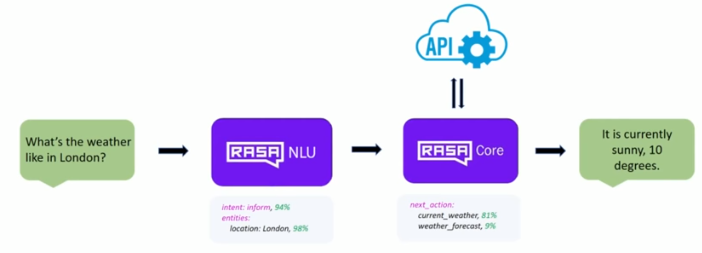
\includegraphics[width=\linewidth]{rasa9}
\end{center}


% {\tiny (Ref: Building a chatbot with Rasa NLU and Rasa Core – jpboost) }

\end{frame}


%%%%%%%%%%%%%%%%%%%%%%%%%%%%%%%%%%%%%%%%%%%%%%%%%%%%%%%%%%%
\begin{frame}[fragile]\frametitle{Like a Human!!}


\begin{center}
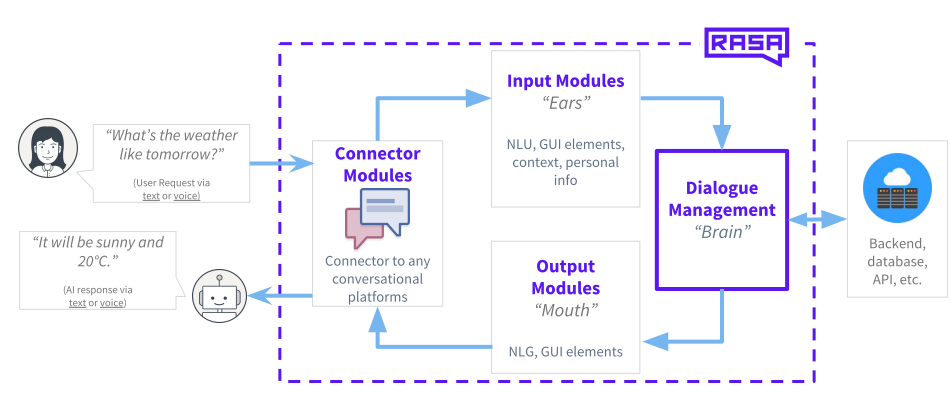
\includegraphics[width=\linewidth]{rasa13}
\end{center}


{\tiny (Ref: Conversational AI: Building clever chatbots - Tom Bocklisch)}

\end{frame}

%%%%%%%%%%%%%%%%%%%%%%%%%%%%%%%%%%%%%%%%%%%%%%%%%%%%%%%%%%%%%%%%%%%%%%%%%%%%%%%%%%
\begin{frame}[fragile]\frametitle{}
\begin{center}

{\Large Rasa NLU: Intents and Entities}

\end{center}
\end{frame}

%%%%%%%%%%%%%%%%%%%%%%%%%%%%%%%%%%%%%%%%%%%%%%%%%%%%%%%%%%%
 \begin{frame}[fragile]\frametitle{RASA NLU Server}
\begin{itemize}
\item A RASA-NLU platform needs to be trained before we start using it. 
\item We need to supply it with a few sentences and mention which are the intents and entities in it.
\end{itemize}
\end{frame}

%%%%%%%%%%%%%%%%%%%%%%%%%%%%%%%%%%%%%%%%%%%%%%%%%%%%%%%%%%%
\begin{frame}[fragile]\frametitle{Natural Language Understanding (NLU)}


\begin{center}
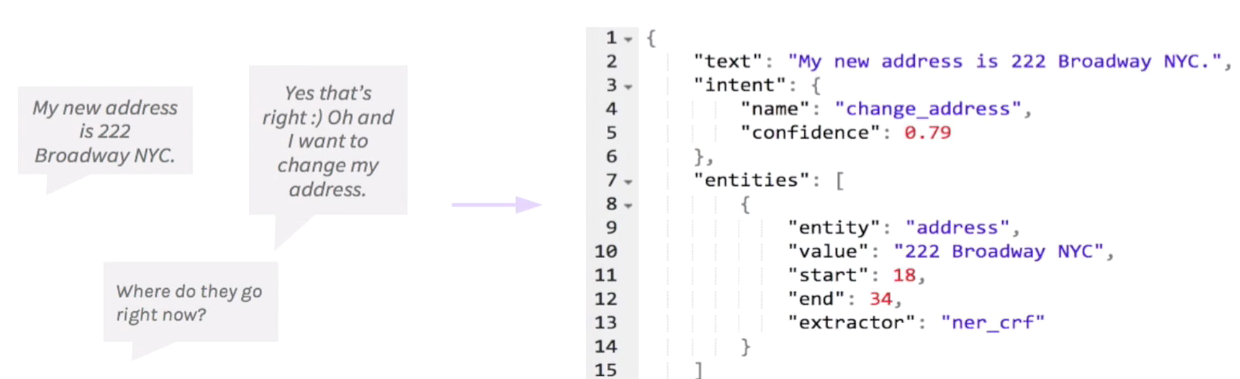
\includegraphics[width=\linewidth]{rasa20}
\end{center}

Goal: take a sentence string, and extract structured information. Decide one from set of predefined intents. Extract entities: types and values.

{\tiny (Ref: Building Conversational AI w Rasa Stack - Alan Nichol  PyBay2018)}

\end{frame}

%%%%%%%%%%%%%%%%%%%%%%%%%%%%%%%%%%%%%%%%%%%%%%%%%%%%%%%%%%%
 \begin{frame}[fragile]\frametitle{Intents}
\begin{itemize}
\item Intents are the actions/categories of the sentences
\item An Intent is a collection of expressions(what the user says) that mean the same thing but are constructed differently. \item Each intent corresponds to one action your user wants to perform.
\item Consider it as the aim or target of the user input. If a user say, ``Which day is today?'', the intent would be finding the day of the week.
\item For example, ``I wish to book a flight from Mumbai to Pune on 27 March'' has ``flight-booking'' as the intent 
\end{itemize}

\begin{center}
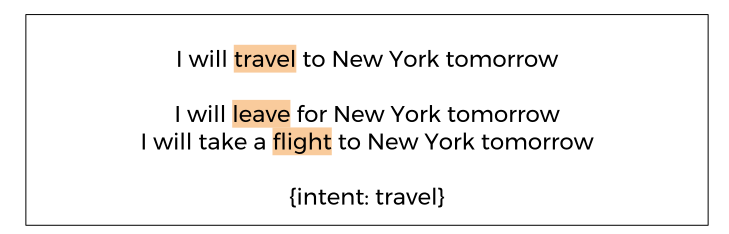
\includegraphics[width=0.6\linewidth]{chatbot53}
\end{center}

\end{frame}


%%%%%%%%%%%%%%%%%%%%%%%%%%%%%%%%%%%%%%%%%%%%%%%%%%%%%%%%%%%
 \begin{frame}[fragile]\frametitle{Intents}
\begin{itemize}
\item For example, An intent ``greet'' will have the following expressions ``hi,'' hello,'' hey,'' all meaning the same thing as a greeting or conversation initiator.
\item The following is an intent training done in dialogflow to get\_meaning of a word.
\end{itemize}

\begin{center}
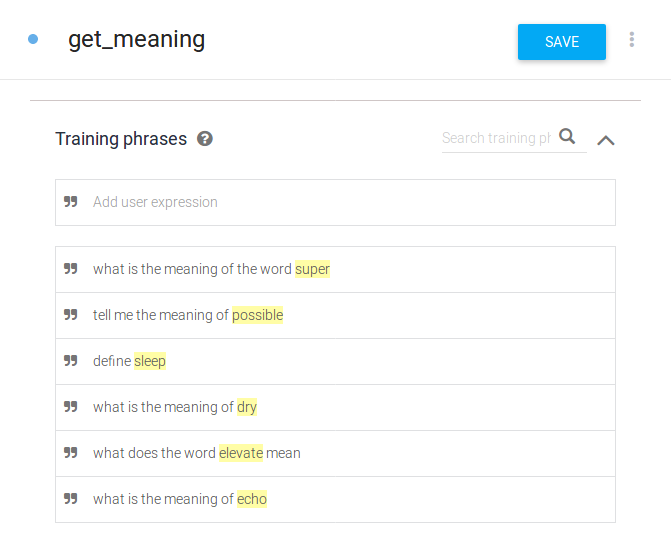
\includegraphics[width=0.5\linewidth,keepaspectratio]{rasa3}
\end{center}

{\tiny (Ref: Chatbots 101 - Architecture \& Terminologies -  Bhavani Ravi)}

\end{frame}


%%%%%%%%%%%%%%%%%%%%%%%%%%%%%%%%%%%%%%%%%%%%%%%%%%%%%%%%%%%
 \begin{frame}[fragile]\frametitle{Entity}
\begin{itemize}
\item Entities are the necessary variables needed to fulfill the actions.
\item An Entity is an information extracted from what a user says. These are the details you want the bot engine to capture in order to perform the action.
\item For the ``flight-booking'' intent, ``Mumbai'',``Pune'' and ``27 March'' as the entities. 
\item Consider it as the useful information from the user input that can be extracted. 
\item From previous example, by intent we understand the aim is to find the day of week, but of which date? If we extract ``Today'' as the entity, we can perform the action on today.
\end{itemize}

\begin{center}
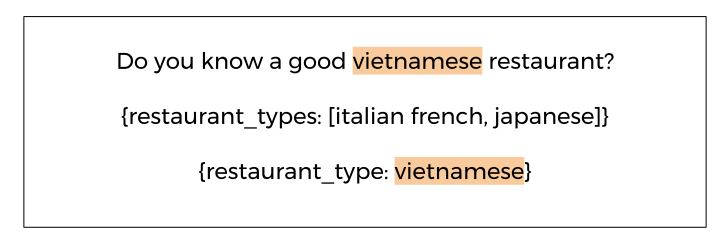
\includegraphics[width=0.6\linewidth]{chatbot54}
\end{center}

\end{frame}

%%%%%%%%%%%%%%%%%%%%%%%%%%%%%%%%%%%%%%%%%%%%%%%%%%%%%%%%%%%
 \begin{frame}[fragile]\frametitle{Entities}
For example, When you look for a famous place in a city you would need to capture information like the kind of place, the city and the personal preferences like timings etc.,


\begin{center}
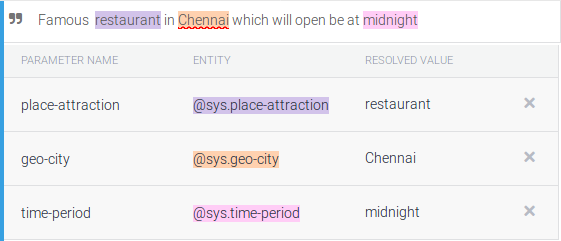
\includegraphics[width=\linewidth,keepaspectratio]{rasa4}
\end{center}

{\tiny (Ref: Chatbots 101 - Architecture \& Terminologies -  Bhavani Ravi)}

\end{frame}


%%%%%%%%%%%%%%%%%%%%%%%%%%%%%%%%%%%%%%%%%%%%%%%%%%%%%%%%%%%
 \begin{frame}[fragile]\frametitle{NLU Training Data}

\begin{center}
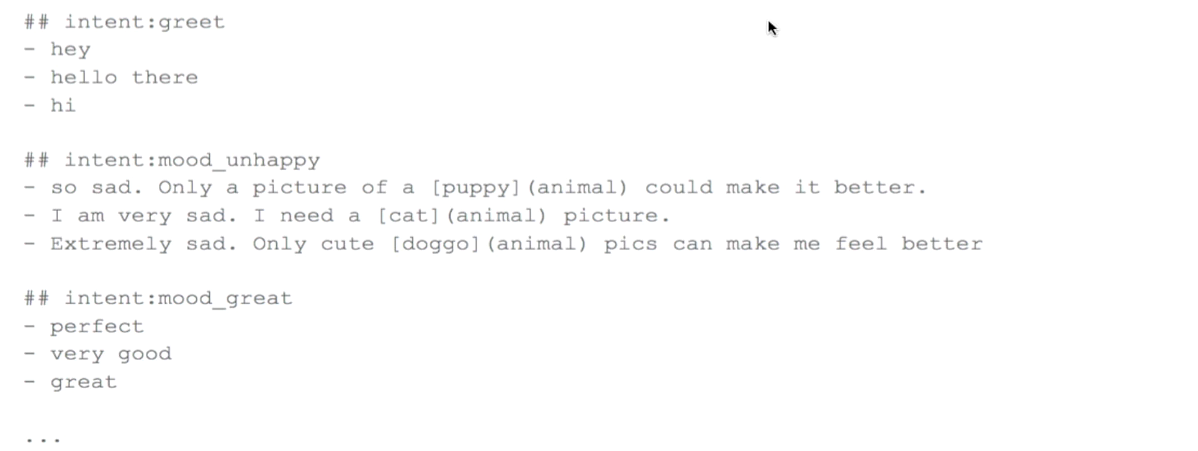
\includegraphics[width=\linewidth,keepaspectratio]{rasa22}
\end{center}

Entities in square brackets and intents in round brackets

{\tiny (Ref: Building Conversational AI w Rasa Stack - Alan Nichol at PyBay2018)}

\end{frame}



%%%%%%%%%%%%%%%%%%%%%%%%%%%%%%%%%%%%%%%%%%%%%%%%%%%%%%%%%%%
 \begin{frame}[fragile]\frametitle{NLU Training Data}
 
Training data is stored in a json, a sample of which can be seen at https://github.com/RASAHQ/rasa\_nlu/blob/master/data/examples/rasa/demo-rasa.json
It contains many entries. One of the sample entries is shown below:
\begin{lstlisting}
{
        "text": "show me a mexican place in the centre",
        "intent": "restaurant_search",
        "entities": [
          {
            "start": 31,
            "end": 37,
            "value": "centre",
            "entity": "location"
          },
          {
            "start": 10,
            "end": 17,
            "value": "mexican",
            "entity": "cuisine"
          }
        ]
}
\end{lstlisting}

\end{frame}

%%%%%%%%%%%%%%%%%%%%%%%%%%%%%%%%%%%%%%%%%%%%%%%%%%%%%%%%%%%
 \begin{frame}[fragile]\frametitle{NLU Training Data}
 Following is the explanation of some of the fields mentioned in the json seen:
\begin{itemize}
\item text: the input sentence.
\item intent: action or category, in this instance ``restaurant\_search''. This is typically the call-back function name.
\item entities: array of entities. Here, there are two. One is of type `location' with value as `centre', whereas the other is of type `cuisine' with value `mexican'. `start' and `end' specify beginning and ending indices of the word in the sentence.
\end{itemize}
You can use the below online tool as well, to generate this json file:

https://rasahq.github.io/rasa-nlu-trainer/
\end{frame}



%%%%%%%%%%%%%%%%%%%%%%%%%%%%%%%%%%%%%%%%%%%%%%%%%%%%%%%%%%%
 \begin{frame}[fragile]\frametitle{NLU Trainer Tool}
\begin{itemize}
\item There is a great tool (rasa\_nlu\_trainer) you can use to add new examples/Intents/entities.
\item 
To install it, run in terminal: \lstinline|npm i -g rasa-nlu-trainer (you'll need nodejs and npm for this)| . For other platforms, need to look around. 
\item Run: \lstinline|rasa-nlu-trainer -v <path to the training data file>|
\item Here is a screenshot of the trainer:

\begin{center}
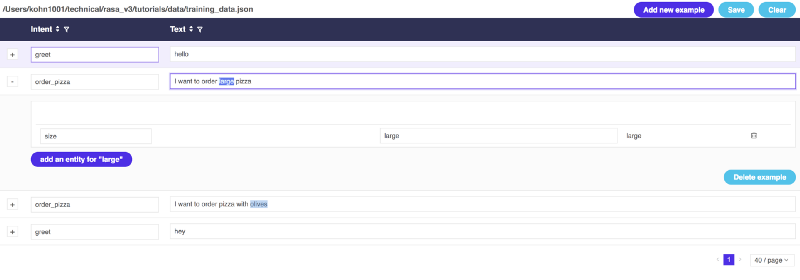
\includegraphics[width=0.8\linewidth,keepaspectratio]{chatbot31}
\end{center}

\item There is one web version too!! https://rasahq.github.io/rasa-nlu-trainer/
\end{itemize}

\end{frame}

%%%%%%%%%%%%%%%%%%%%%%%%%%%%%%%%%%%%%%%%%%%%%%%%%%%%%%%%%%%
 \begin{frame}[fragile]\frametitle{NLU Training}
\begin{itemize}
\item The training part generates an ML model when you feed the training data
\item This training can be either by python program or by command line
\end{itemize}

\end{frame}

%%%%%%%%%%%%%%%%%%%%%%%%%%%%%%%%%%%%%%%%%%%%%%%%%%%%%%%%%%%
 \begin{frame}[fragile]\frametitle{NLU Training by Command Line}
\begin{itemize}
\item Training:
\begin{lstlisting}
$ python -m rasa_nlu.train \
    --config sample_configs/config_spacy.yml \
    --data data/examples/rasa/demo-rasa.json \
    --path projects
\end{lstlisting}
\item Serving:
\begin{lstlisting}
$ python -m rasa_nlu.server --path projects
\end{lstlisting}
\item Here ``projects'' is the model name
\end{itemize}

\end{frame}

%%%%%%%%%%%%%%%%%%%%%%%%%%%%%%%%%%%%%%%%%%%%%%%%%%%%%%%%%%%
 \begin{frame}[fragile]\frametitle{Training NLU by Python Script}
 
\begin{lstlisting}
from rasa_nlu.training_data import load_data
from rasa_nlu.config import RasaNLUModelConfig
from rasa_nlu.model import Trainer
from rasa_nlu import config
from rasa_nlu.model import Metadata, Interpreter

def train (data, config_file, model_dir):
    training_data = load_data(data)
    trainer = Trainer(config.load(config_file))
    trainer.train(training_data)
    model_directory = trainer.persist(model_dir, fixed_model_name = 'chat')

train('data/nlu_train.md', 'nlu_config.yml', 'models/nlu'
\end{lstlisting}
This will train the nlu model and save it at `models/nlu/'.
\end{frame}

%%%%%%%%%%%%%%%%%%%%%%%%%%%%%%%%%%%%%%%%%%%%%%%%%%%%%%%%%%%
 \begin{frame}[fragile]\frametitle{Testing NLU model by Python Script}
 
Lets try and test how is the model working.

\begin{lstlisting}
interpreter = Interpreter.load('./models/nlu/default/chat')

def ask_question(text):
    print(interpreter.parse(text))

ask_question("How many days in January")
ask_question("How many days in March
\end{lstlisting}

\end{frame}

%%%%%%%%%%%%%%%%%%%%%%%%%%%%%%%%%%%%%%%%%%%%%%%%%%%%%%%%%%%
 \begin{frame}[fragile]\frametitle{Testing NLU model}
The output looks something like this,


\begin{lstlisting}
{'intent': {'name': 'query_days_in_month', 'confidence': 0.6128492334410716}, 'entities': [{'start': 17, 'end': 24, 'value': 'january', 'entity': 'month', 'confidence': 0.5002208121139594, 'extractor': 'ner_crf'}], 'intent_ranking': [{'name': 'query_days_in_month', 'confidence': 0.6128492334410716}, {'name': 'bye', 'confidence': 0.1951941314517159}, {'name': 'greet', 'confidence': 0.19195663510721267}], 'text': 'How many days in January'}

{'intent': {'name': 'query_days_in_month', 'confidence': 0.6105606961005596}, 'entities': [{'start': 17, 'end': 22, 'value': 'march', 'entity': 'month', 'confidence': 0.5002208121139594, 'extractor': 'ner_crf'}], 'intent_ranking': [{'name': 'query_days_in_month', 'confidence': 0.6105606961005596}, {'name': 'bye', 'confidence': 0.20686031746694789}, {'name': 'greet', 'confidence': 0.18257898643249237}], 'text': 'How many days in March'
\end{lstlisting}

\end{frame}

%%%%%%%%%%%%%%%%%%%%%%%%%%%%%%%%%%%%%%%%%%%%%%%%%%%%%%%%%%%
 \begin{frame}[fragile]\frametitle{Testing NLU model}

\begin{itemize}
\item Here as you can see, the model was perfectly able to tag the user question to it's intent (check `name` section under `intent`). 
\item It says, that for the first question, the intent was `query\_days\_in\_month` and the extracted entity was `January` (check `value'under `entities`). 
\item One cool thing is in the output of second question, even though we didn't provide this in example, it was perfectly able to guess the intent and even extract the entity `march`.
\end{itemize}
\end{frame}

%%%%%%%%%%%%%%%%%%%%%%%%%%%%%%%%%%%%%%%%%%%%%%%%%%%%%%%%%%%%%%%%%%%%%%%%%%%%%%%%%%
\begin{frame}[fragile]\frametitle{}
\begin{center}
{\Large Rasa Core: Dialog Management}
\end{center}
\end{frame}


%%%%%%%%%%%%%%%%%%%%%%%%%%%%%%%%%%%%%%%%%%%%%%%%%%%%%%%%%%%
 \begin{frame}[fragile]\frametitle{RASA Core: Actions and Stories}
\begin{itemize}
\item The job of Rasa Core is to essentially generate the reply message for the chatbot. 
\item It takes the output of Rasa NLU (intent and entities) and applies Machine Learning models to generate a reply.
\end{itemize}

\begin{center}
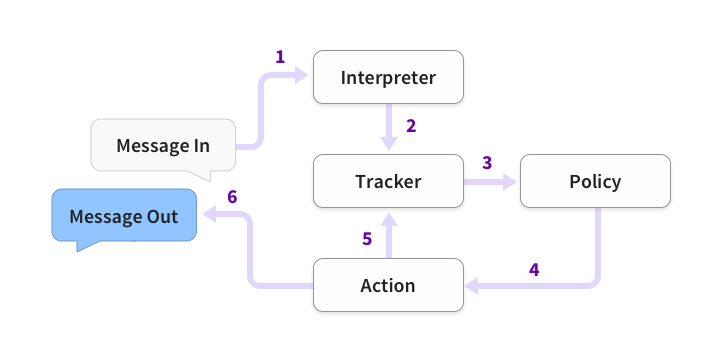
\includegraphics[width=0.5\linewidth,keepaspectratio]{rasa1}
\end{center}

\begin{itemize}
\item The input message is interpreted by an Interpreter to extract intent and entity. 
\item It is then passed to the Tracker that keeps track of the current state of the conversation. 
\item The Policy applies Machine Learning algorithm to determine what should be the reply and choses Action accordingly.
\item Action updates the Tracker to reflect the current state.
\end{itemize}

\end{frame}


%%%%%%%%%%%%%%%%%%%%%%%%%%%%%%%%%%%%%%%%%%%%%%%%%%%%%%%%%%%
 \begin{frame}[fragile]\frametitle{Actions}
\begin{itemize}
\item Its an operation which can be performed by the bot. 
\item It could be replying something in return, querying a database or any other thing possible by code.
\item So, an Action is a task that you expect your bot to do. 
\item In most cases, An external API performs this action. Since the bot platforms do not support external API calls, An external program is used to drive that functionality.
\item For example, When you ask your bot to order pizza for you, the bot extracts all the information(Entities) required to order pizza say, size, type, topping etc and sends it to an external API and gets a response whether the order is successful or not.

\end{itemize}

{\tiny (Ref: Chatbots 101 - Architecture \& Terminologies -  Bhavani Ravi)}

\end{frame}

%%%%%%%%%%%%%%%%%%%%%%%%%%%%%%%%%%%%%%%%%%%%%%%%%%%%%%%%%%%
 \begin{frame}[fragile]\frametitle{Actions}
\begin{itemize}
\item Actions are either utterances, which means, the output that we want to send the user, or you can actually create your own class that inherent form Action. 
\item Say: ``actions.ActionOrderPizza'', here again Rasa has a very cool interface, you should inherent from Class Action and add your logic in the derived class according to what you need, here is an example, create the file action.py (just a stub below):
\begin{lstlisting}
from rasa_core.actions import Action

class ActionOrderPizza(Action):
    def name(self):
        return 'action_order_pizza'
    def run(self):
        print('Ordering Pizza is completed! It should be with you soon :)')
        pass
\end{lstlisting}
\end{itemize}

\end{frame}


%%%%%%%%%%%%%%%%%%%%%%%%%%%%%%%%%%%%%%%%%%%%%%%%%%%%%%%%%%%
 \begin{frame}[fragile]\frametitle{Dialog Stories Data}
\begin{itemize}
\item Rasa core's next state prediction is not flow chart based but machine learning based. 
\item It uses current context, intents, current state in the conversation, etc to decide next steps.
\item You need to give some samples of interactions, in form of stories.
\item These are a sample interaction between the user and bot, defined in terms of intents captured and actions performed. 
\item So developer can mention what to do if you get a use input of some intent with/without some entities. 
\item Like saying if user intent is to find the day of week and entity is today, find day of week of today and reply.
\end{itemize}

To make this work, Rasa need some files, which stores all the training and model information to build the bot.
\end{frame}

%%%%%%%%%%%%%%%%%%%%%%%%%%%%%%%%%%%%%%%%%%%%%%%%%%%%%%%%%%%
 \begin{frame}[fragile]\frametitle{Dialog Stories Data}

Contains a bunch of stories to learn from. From each stories, creates a probability model of interactions.

\begin{center}
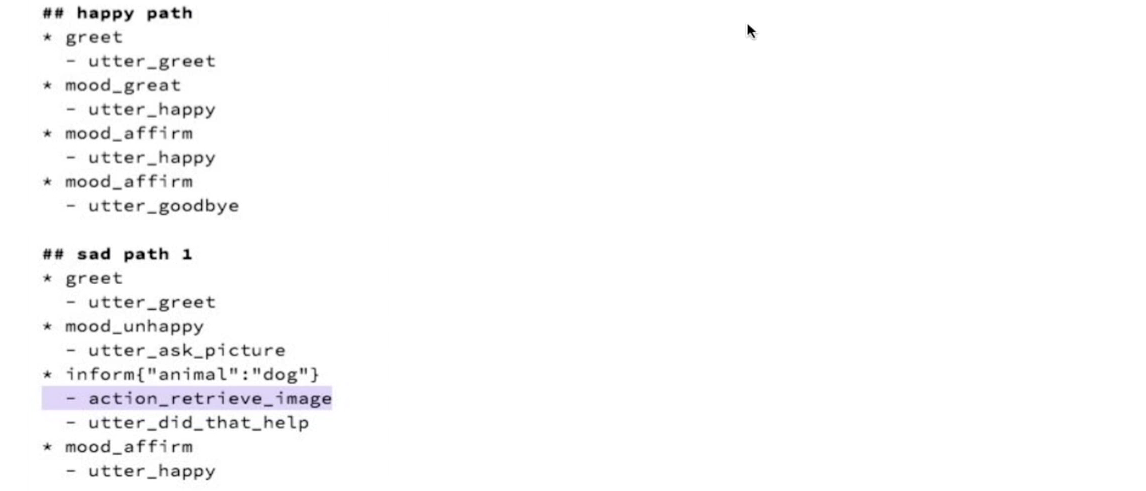
\includegraphics[width=\linewidth,keepaspectratio]{rasa23}
\end{center}

\begin{itemize}
\item Simplest actions are utterances (template-ed fixed response strings)
\item More flexible are the ones called "actions\_" for API calls
\end{itemize}

{\tiny (Ref: Building Conversational AI w Rasa Stack - Alan Nichol at PyBay2018)}

\end{frame}


%%%%%%%%%%%%%%%%%%%%%%%%%%%%%%%%%%%%%%%%%%%%%%%%%%%%%%%%%%%
 \begin{frame}[fragile]\frametitle{Dialog Stories Data}
Lets create a sample user-bot interaction.

stories.md
\begin{lstlisting}
## story1              
* greet              
  - utter_greet
* query_days_in_month{"month":"January"}
  - utter_answer_31_days
* query_days_in_month{"month":"February"}
  - utter_answer_28_days
* query_days_in_month{"month":"April"}
  - utter_answer_30_days
* bye               
  - utter_bye
\end{lstlisting}

\begin{itemize}
\item Here we are defining a sample interaction between the bot and user in form of a story. 
\item It goes like this, if user says something and its intent is `greet` bot will perform action `utter\_greet`. 
\item One more example, if user's message has `query\_days\_in\_month` intent and `February' then bot will perform `utter\_answer\_28\_days` action.
\end{itemize}
\end{frame}

%%%%%%%%%%%%%%%%%%%%%%%%%%%%%%%%%%%%%%%%%%%%%%%%%%%%%%%%%%%
 \begin{frame}[fragile]\frametitle{Training Dialog Data}
Lets train the dialog management part,

\begin{lstlisting}
def train_dialog(dialog_training_data_file, domain_file, path_to_model = 'models/dialogue'):
    logging.basicConfig(level='INFO')
    agent = Agent(domain_file,
              policies=[MemoizationPolicy(max_history=1)])
    training_data = agent.load_data(dialog_training_data_file)
    agent.train(
        training_data,
        augmentation_factor=50,
        epochs=200,
        batch_size=10,
        validation_split=0.2)
    agent.persist(path_to_model)

train_dialog('data/stories.md', 'domain.yml')
\end{lstlisting}

\end{frame}


%%%%%%%%%%%%%%%%%%%%%%%%%%%%%%%%%%%%%%%%%%%%%%%%%%%%%%%%%%%
 \begin{frame}[fragile]\frametitle{Training Policy}

\begin{itemize}
\item Here, you can change the training policy in which you can define your own LSTM or RNN for dialog training. 
\item One important point, `max\_history` is used to define how one action is dependent on previous questions. 
\item If max\_history is 1, then it just memorizes individual intent and its related actions. Due to lack of training data (huge load of stories), I am just making it memorize the rules now, you can create some sample stories and see the true potential of rasa dialog management.
\end{itemize}
\end{frame}

%%%%%%%%%%%%%%%%%%%%%%%%%%%%%%%%%%%%%%%%%%%%%%%%%%%%%%%%%%%
 \begin{frame}[fragile]\frametitle{Testing}
Lets see if the bot is able to reply back to us and answers our question.

\begin{lstlisting}
# Loading the Agent
rasaNLU = RasaNLUInterpreter("models/nlu/default/chat")
agent = Agent.load("models/dialogue", interpreter= rasaNLU)

# asking question
agent.handle_message('Hi')
>>> [{'recipient_id': 'default', 'text': 'Hey'}]

# once more
agent.handle_message('How many days in January')
>>> [{'recipient_id': 'default', 'text': 'There are 31 days in the mentioned month.'}]

# once more
agent.handle_message('How many days in April')
>>> [{'recipient_id': 'default', 'text': 'There are 30 days in the mentioned month.'}]

# once more
agent.handle_message('Bye')
>>> [{'recipient_id': 'default', 'text': 'Goodbye'}]
\end{lstlisting}

And it does!
\end{frame}

%%%%%%%%%%%%%%%%%%%%%%%%%%%%%%%%%%%%%%%%%%%%%%%%%%%%%%%%%%%
 \begin{frame}[fragile]\frametitle{Observations}

\begin{itemize}
\item Mapping every combination of intent-entity to its action in stories is quite inefficient. Just think of individually mapping each month to its answer. This could be handled by using custom actions, where the action calls a python function with all the info like the intent and entity.
\item The true potential of the rasa nlu and core shines when you give it more data to train.
\end{itemize}
\end{frame}


%%%%%%%%%%%%%%%%%%%%%%%%%%%%%%%%%%%%%%%%%%%%%%%%%%%%%%%%%%%
 \begin{frame}[fragile]\frametitle{Online Training the Dialog}
 Can stories be created by saving online interactions?
 
online\_train.py:
\begin{lstlisting}
def run_online_trainer(input_channel,
                        interpreter,
                        domain_def_file='chat_domain.yml',
                        training_data_file='./data/stories.md'):
    agent = Agent(  domain_def_file,
                    policies=[KerasPolicy(), MemoizationPolicy()],
                    interpreter=interpreter)
    agent.train_online( training_data_file,
                        input_channel=input_channel,
                        max_history=2,
                        batch_size=500,
                        epochs=200,
                        max_training_samples=300)
    return agent
if __name__ == '__main__':
    logging.basicConfig(level='INFO')
    interpreter = RasaNLUInterpreter('./models/nlu/default/chat')
    run_online_trainer(ConsoleInputChannel(), interpreter)
\end{lstlisting}

Run by \lstinline|python online_train.py|

\end{frame}


%%%%%%%%%%%%%%%%%%%%%%%%%%%%%%%%%%%%%%%%%%%%%%%%%%%%%%%%%%%
 \begin{frame}[fragile]\frametitle{Online Training the Dialog}
You should get an interactive session in which you should follow the expected flow, for example:
 
\begin{center}
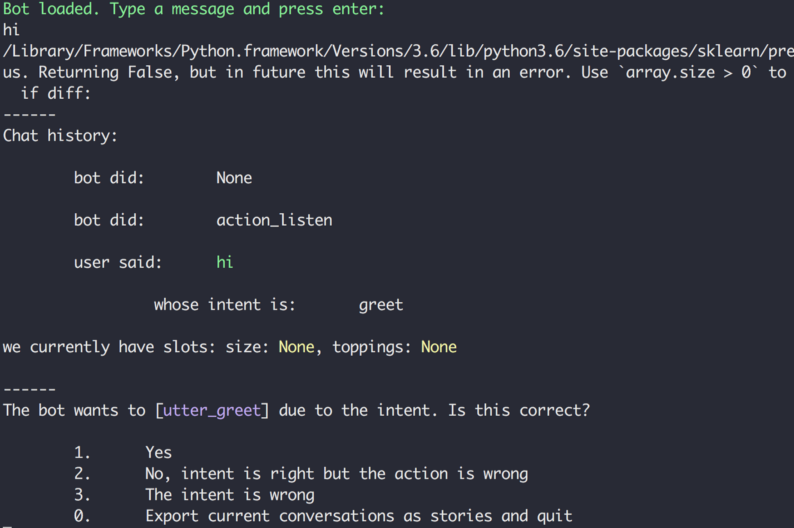
\includegraphics[width=0.6\linewidth]{chatbot32}
\end{center}

\begin{itemize}
\item In the first green line it says that the bot has been loaded and is waiting for the user input.
\item Next we type: ``hi''
\item Now you can see that the system prints the ``Chat history'':
\begin{itemize}
\item we can see that the flow is correct:
\item bot did: action\_listen
\item user said: hi
\item whose intent is: greet
\end{itemize}
\end{itemize}

\end{frame}

%%%%%%%%%%%%%%%%%%%%%%%%%%%%%%%%%%%%%%%%%%%%%%%%%%%%%%%%%%%
 \begin{frame}[fragile]\frametitle{Online Training the Dialog}
\begin{itemize}
\item Now the system is waiting for your feedback, in this case the flow is correct, so we should type: 2.
\item You can continue doing this as long as you want, when you finish type ``0'' to export the new stories.md file (give it new name, such: ``stories\_v1.md'').
\item Now replace the previous stories file (back it up first!) or concatenate them in the same stories file, that way you should have more and more training data!
\end{itemize}

\end{frame}



%%%%%%%%%%%%%%%%%%%%%%%%%%%%%%%%%%%%%%%%%%%%%%%%%%%%%%%%%%%%%%%%%%%%%%%%%%%%%%%%%%
\begin{frame}[fragile]\frametitle{}
\begin{center}
{\Large Config Files}

% {\tiny (Ref: Building a chatbot with Rasa - Mohit Mayank )}
\end{center}
\end{frame}

%%%%%%%%%%%%%%%%%%%%%%%%%%%%%%%%%%%%%%%%%%%%%%%%%%%%%%%%%%%
 \begin{frame}[fragile]\frametitle{Config file}
 
 The training configuration is defined as below . It contains two main info language of your bot and the NLP library to use.
 
 
nlu\_config.yml


\begin{lstlisting}
pipeline: "spacy_sklearn"
language: "en"
\end{lstlisting}

We will define the pipeline to use for training the NLU model, here we will use spacy to do so.
\end{frame}

%%%%%%%%%%%%%%%%%%%%%%%%%%%%%%%%%%%%%%%%%%%%%%%%%%%%%%%%%%%
 \begin{frame}[fragile]\frametitle{Domain file}
 
\begin{itemize}
\item Here you list all of the intents, entities, actions and similar information. 
\item You can also add sample bot reply templates and use them as actions.
\end{itemize}

\begin{center}
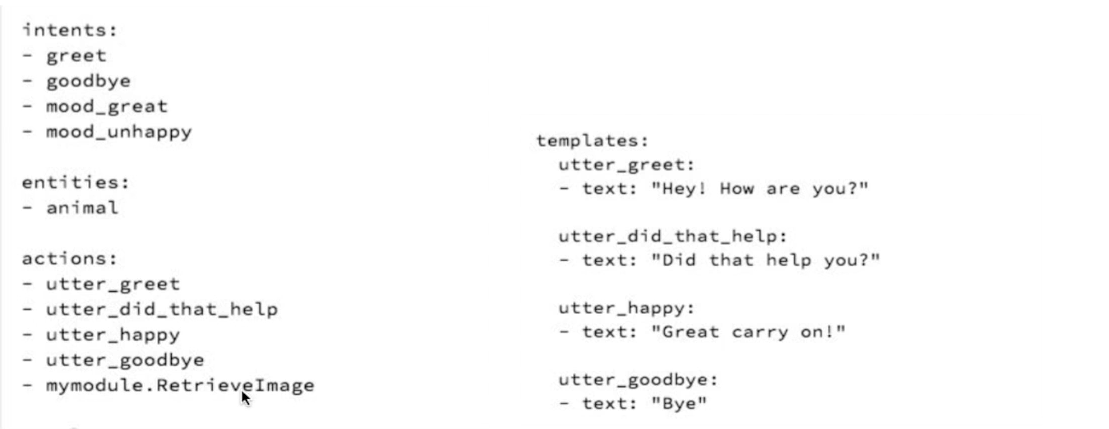
\includegraphics[width=\linewidth,keepaspectratio]{rasa24}
\end{center}

Custom action shown above is to be written in a separate file (elaborated later)


{\tiny (Ref: Building Conversational AI w Rasa Stack - Alan Nichol at PyBay2018)}

\end{frame}




% %%%%%%%%%%%%%%%%%%%%%%%%%%%%%%%%%%%%%%%%%%%%%%%%%%%%%%%%%%%%%%%%%%%%%%%%%%%%%%%%%%
% \begin{frame}[fragile]\frametitle{}
% \begin{center}
% {\Large Files}

% {\tiny (Ref: Building a chatbot with Rasa - Mohit Mayank )}
% \end{center}
% \end{frame}


% %%%%%%%%%%%%%%%%%%%%%%%%%%%%%%%%%%%%%%%%%%%%%%%%%%%%%%%%%%%
 % \begin{frame}[fragile]\frametitle{RASA NLU Implementation}
 % RasaNLU has two entry points: Train and Server.
% \begin{itemize}
% \item The training part generates an ML model when you feed the training data: train.py
% \begin{lstlisting}
% python -m rasa_nlu.train \
    % --config sample_configs/config_spacy.yml \
    % --data data/examples/rasa/demo-rasa.json \
    % --path projects
% \end{lstlisting}
% \item The server part is where the generated ML model is served via an API
% \begin{lstlisting}
% python -m rasa_nlu.server --path projects
% \end{itemize}
% \end{lstlisting}

% {\tiny (Ref: NLP Behind Chatbots—Demystifying RasaNLU - Bhavani Ravi )}

% \end{frame}


% %%%%%%%%%%%%%%%%%%%%%%%%%%%%%%%%%%%%%%%%%%%%%%%%%%%%%%%%%%%%%%%%%%%%%%%%%%%%%%%%%%
% \begin{frame}[fragile]\frametitle{}
% \begin{center}
% {\Large Training}
% \end{center}
% \end{frame}



%%%%%%%%%%%%%%%%%%%%%%%%%%%%%%%%%%%%%%%%%%%%%%%%%%%%%%%%%%%
 \begin{frame}[fragile]\frametitle{Domain file}
Define domain file which contains sample templates to reply back to user.

domain.yml
\begin{lstlisting}
intents:
# place your intents
 - greet
 - query_days_in_month
 - bye
entities:
# place your entities
 - month
templates:
# sample replies
 utter_greet:
  - "Hey, how can I help you?"
 utter_answer_31_days:
  - "There are 31 days in the mentioned month."
 utter_answer_30_days:
  - "There are 30 days in the mentioned month."
 utter_answer_28_days:
  - "There are 28 days in the mentioned month."
 utter_bye:
  - "Goodbye"
\end{lstlisting}
\end{frame}

%%%%%%%%%%%%%%%%%%%%%%%%%%%%%%%%%%%%%%%%%%%%%%%%%%%%%%%%%%%
 \begin{frame}[fragile]\frametitle{Domain file}
domain.yml (continued)
\begin{lstlisting}
actions:
# templates (as they are reply actions),
# also custom actions if any
 - utter_greet
 - utter_answer_31_days
 - utter_answer_30_days
 - utter_answer_28_days
 - utter_bye
\end{lstlisting}

\begin{itemize}
\item Here we have listed down the intents and entities (all present in nlu training file), along with some templates and actions. 
\item Templates contains replies that you want the bot to make, in this case I want the bot to greet, say goodbye and also answer the user asked question of number of days in the month. 
\item And right now bot will only answer these three types of month answers (bot is agnostic of leap years, stupid bot)
\end{itemize}
\end{frame}


%%%%%%%%%%%%%%%%%%%%%%%%%%%%%%%%%%%%%%%%%%%%%%%%%%%%%%%%%%%%%%%%%%%%%%%%%%%%%%%%%%
\begin{frame}[fragile]\frametitle{}
\begin{center}
{\Large Sample Conversation flow}

\end{center}
\end{frame}


%%%%%%%%%%%%%%%%%%%%%%%%%%%%%%%%%%%%%%%%%%%%%%%%%%%%%%%%%%%
\begin{frame}[fragile]\frametitle{Chatbot Workflow}

Say, you want interaction like below, (go from bottom to top, alternate, right, left)

\begin{center}
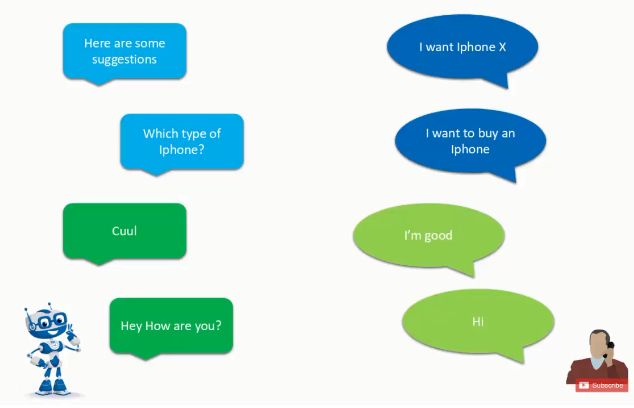
\includegraphics[width=0.7\linewidth]{rasa5}
\end{center}

How do you build this interaction flow?

% {\tiny (Ref: Rasa NLU & Rasa Core Tutorial - Building Chatbots – J-Secur1ty )}

\end{frame}


%%%%%%%%%%%%%%%%%%%%%%%%%%%%%%%%%%%%%%%%%%%%%%%%%%%%%%%%%%%
\begin{frame}[fragile]\frametitle{Stories, Paths}

Happy path and Sad path

\begin{center}
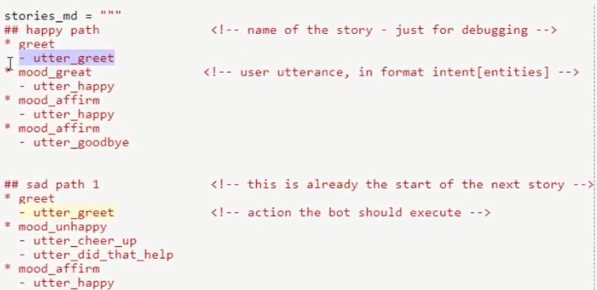
\includegraphics[width=\linewidth]{rasa6}
\end{center}


% {\tiny (Ref: Rasa NLU & Rasa Core Tutorial - Building Chatbots – J-Secur1ty )}

\end{frame}


%%%%%%%%%%%%%%%%%%%%%%%%%%%%%%%%%%%%%%%%%%%%%%%%%%%%%%%%%%%
\begin{frame}[fragile]\frametitle{Stories, Paths}

Purchase path

\begin{center}
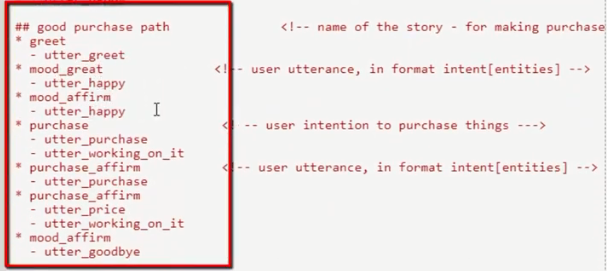
\includegraphics[width=\linewidth]{rasa7}
\end{center}


% {\tiny (Ref: Rasa NLU & Rasa Core Tutorial - Building Chatbots – J-Secur1ty )}

\end{frame}

%%%%%%%%%%%%%%%%%%%%%%%%%%%%%%%%%%%%%%%%%%%%%%%%%%%%%%%%%%%
\begin{frame}[fragile]\frametitle{Domain}

Domain contains everything

\begin{center}
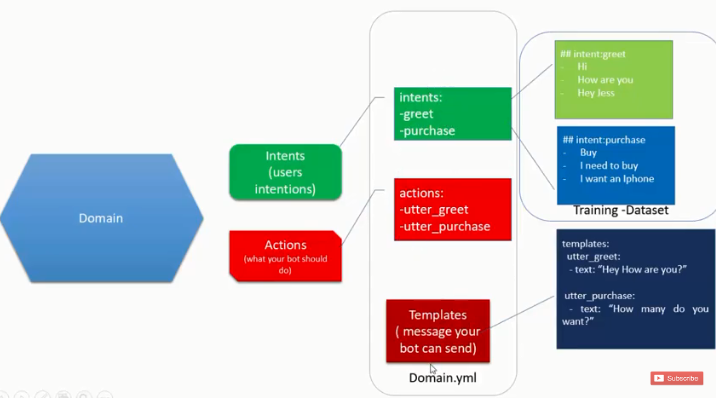
\includegraphics[width=\linewidth]{rasa8}
\end{center}


% {\tiny (Ref: Rasa NLU & Rasa Core Tutorial - Building Chatbots – J-Secur1ty )}

\end{frame}


%%%%%%%%%%%%%%%%%%%%%%%%%%%%%%%%%%%%%%%%%%%%%%%%%%%%%%%%%%%
\begin{frame}[fragile]\frametitle{What's Next?}
How these modules work? 

Can dig deep, to find that these are all Machine Learning techniques!!

Can you guess a few?

\end{frame}
